\documentclass[11pt,a4paper]{article}

\usepackage{fontspec}
\setmainfont{Times New Roman}
\usepackage[russian]{babel}

\usepackage[left=20mm,right=15mm,top=15mm,bottom=15mm]{geometry}
\usepackage{amsmath,amssymb,amsfonts}
\usepackage{graphicx}
\usepackage{booktabs}
\usepackage{array}
\usepackage{caption}
\usepackage{hyperref}
\usepackage{microtype}
\usepackage{float}

\hypersetup{
    colorlinks=true,
    linkcolor=black,
    urlcolor=blue,
    citecolor=black
}

\setlength{\parindent}{1.25cm}
\setlength{\parskip}{0.15em}
\linespread{1.1}
\setlength{\abovedisplayskip}{3pt}
\setlength{\belowdisplayskip}{3pt}

\begin{document}

% -------------------------------------------------------------
% ТИТУЛЬНЫЙ ЛИСТ
% -------------------------------------------------------------
\begin{titlepage}
    \centering
    {\bfseries\large Белорусский государственный университет\par}
    {\bfseries\large Факультет прикладной математики и информатики\par}
    
    \vspace{6cm}
    {\Huge\bfseries ОТЧЁТ\par}
    \vspace{0.5cm}
    {\large по бонусной лабораторной работе по компьютерной графике\par}
    \vspace{0.5cm}
    {\Large\bfseries Формирование, трёхмерные преобразования и визуализация 3D-объекта с текстурой\par}
    
    \vspace{6cm}
    \begin{flushright}
        \large
        \textbf{Выполнил:}\\
        студент 4 группы 3 курса\\
        Дикан Д.~А.\\[1em]
        \textbf{Преподаватель:}\\
        старший преподаватель\\
        Соловей Сергей Сергеевич
    \end{flushright}
    
    \vfill
    {\large Минск, 2026\par}
\end{titlepage}

\newpage

% -------------------------------------------------------------
% СТРАНИЦА 2: ЦЕЛЬ И ФОРМИРОВАНИЕ 3D-МОДЕЛИ
% -------------------------------------------------------------
\section*{1. Цель работы}
Изучить и реализовать методы задания трёхмерных объектов с помощью массива координат вершин, применения матричных аффинных преобразований в однородных координатах и наложения растровых текстур. Разработать веб-приложение, которое формирует и визуализирует трёхмерную модель фамилии студента с текстурой и выводит итоговую матрицу преобразования $4 \times 4$ при выполнении трёхмерных преобразований.

\section*{2. Формирование 3D-модели фамилии ДИКАН}
В качестве трёхмерного объекта в модуле \texttt{processing.py} функцией \texttt{build\_dikan\_mesh()} формируется объёмная надпись \textbf{ДИКАН}. Геометрия каждой буквы составлена из набора непересекающихся выпуклых четырёхугольных призм, выдавленных вдоль оси $Z$ на глубину $z \in [-0.80;\ +0.80]$ и отцентрированных относительно начала координат $(0, 0, 0)$ со смещением $c_x = 11.60$, $c_y = 2.10$:
\begin{itemize}
    \item буква \textbf{Д}~--- 6 призм (две нижние лапки, горизонтальное основание, наклонная левая ножка, вертикальная правая стойка и верхняя перекладина);
    \item буква \textbf{И}~--- 3 призмы (две вертикальные стойки и диагональная перемычка);
    \item буква \textbf{К}~--- 4 призмы (левая стойка, центральная перемычка, верхняя и нижняя наклонные ветви);
    \item буква \textbf{А}~--- 3 призмы (две наклонные ножки и горизонтальная перекладина);
    \item буква \textbf{Н}~--- 3 призмы (две вертикальные стойки и горизонтальная перемычка).
\end{itemize}

Всего модель состоит из \textbf{19 объёмных призм} (каждая содержит 8 вершин, 12 треугольников с обходом против часовой стрелки и 12 контурных рёбер):
\begin{itemize}
    \item \textbf{массив вершин \texttt{vertices}:} 152 трёхмерные координаты $(x, y, z)$;
    \item \textbf{массив граней \texttt{triangles}:} 228 треугольников, заданных индексами вершин $[i_0, i_1, i_2]$, текстурными координатами $(u, v)$ и единичными внешними нормалями;
    \item \textbf{массив рёбер \texttt{edges}:} 228 контурных рёбер для отрисовки каркаса.
\end{itemize}

В таблице 1 приведён фрагмент исходного массива координат вершин (первые 8 вершин~--- левая нижняя лапка буквы Д).

\begin{table}[H]
\centering
\caption{Фрагмент исходного массива вершин модели ДИКАН}
\begin{tabular}{@{}rrrrl@{}}
\toprule
\textbf{Индекс} & \textbf{$X$} & \textbf{$Y$} & \textbf{$Z$} & \textbf{Принадлежность} \\
\midrule
0 & $-11.60$ & $-2.90$ & $0.80$  & Передняя грань \\
1 & $-10.75$ & $-2.90$ & $0.80$  & Передняя грань \\
2 & $-10.75$ & $-2.10$ & $0.80$  & Передняя грань \\
3 & $-11.60$ & $-2.10$ & $0.80$  & Передняя грань \\
4 & $-11.60$ & $-2.90$ & $-0.80$ & Задняя грань \\
5 & $-10.75$ & $-2.90$ & $-0.80$ & Задняя грань \\
6 & $-10.75$ & $-2.10$ & $-0.80$ & Задняя грань \\
7 & $-11.60$ & $-2.10$ & $-0.80$ & Задняя грань \\
\bottomrule
\end{tabular}
\end{table}

\newpage

% -------------------------------------------------------------
% СТРАНИЦА 3: МАТРИЦЫ ПРЕОБРАЗОВАНИЙ И АРХИТЕКТУРА
% -------------------------------------------------------------
\section*{3. Трёхмерные преобразования и итоговая матрица $4 \times 4$}
В трёхмерном пространстве масштабирование и повороты являются линейными преобразованиями и представимы матрицами $3 \times 3$, однако параллельный перенос ($x' = x + t_x$) нелинеен. Использование \textbf{однородных координат} $v = [x,\ y,\ z,\ 1]^T$ позволяет объединить все аффинные преобразования в единое матричное умножение размера $4 \times 4$.

Элементарные матрицы преобразований имеют вид:
\begin{equation}
    S(s_x, s_y, s_z) = \begin{pmatrix}
        s_x & 0 & 0 & 0 \\
        0 & s_y & 0 & 0 \\
        0 & 0 & s_z & 0 \\
        0 & 0 & 0 & 1
    \end{pmatrix}, \quad
    T(t_x, t_y, t_z) = \begin{pmatrix}
        1 & 0 & 0 & t_x \\
        0 & 1 & 0 & t_y \\
        0 & 0 & 1 & t_z \\
        0 & 0 & 0 & 1
    \end{pmatrix},
\end{equation}
\begin{equation}
    R_x(\alpha) = \begin{pmatrix}
        1 & 0 & 0 & 0 \\
        0 & \cos\alpha & -\sin\alpha & 0 \\
        0 & \sin\alpha & \cos\alpha & 0 \\
        0 & 0 & 0 & 1
    \end{pmatrix}, \quad
    R_y(\beta) = \begin{pmatrix}
        \cos\beta & 0 & \sin\beta & 0 \\
        0 & 1 & 0 & 0 \\
        -\sin\beta & 0 & \cos\beta & 0 \\
        0 & 0 & 0 & 1
    \end{pmatrix},
\end{equation}
\begin{equation}
    R_z(\gamma) = \begin{pmatrix}
        \cos\gamma & -\sin\gamma & 0 & 0 \\
        \sin\gamma & \cos\gamma & 0 & 0 \\
        0 & 0 & 1 & 0 \\
        0 & 0 & 0 & 1
    \end{pmatrix}.
\end{equation}

Итоговая матрица преобразования вычисляется путём перемножения элементарных матриц в порядке:
\begin{equation}
    M = T(t_x, t_y, t_z) \cdot R_z(\gamma) \cdot R_y(\beta) \cdot R_x(\alpha) \cdot S(s_x, s_y, s_z).
\end{equation}

Позиция каждой вершины модели после преобразования определяется произведением $v' = M \cdot v$: объект сначала масштабируется и поворачивается вокруг собственного центра $(0, 0, 0)$, а затем переносится на вектор $(t_x, t_y, t_z)$. Например, при поворотах $R_x = 28^\circ$, $R_y = 22^\circ$, $R_z = 0^\circ$, переносе $T = (1.5, -0.5, 0.5)$ и масштабе $S = (1, 1, 1)$ итоговая матрица $M$ принимает вид:
\begin{equation}
    M = \begin{pmatrix}
        0.927 & 0.176 & 0.331 & 1.500 \\
        0.000 & 0.883 & -0.469 & -0.500 \\
        -0.375 & 0.435 & 0.819 & 0.500 \\
        0.000 & 0.000 & 0.000 & 1.000
    \end{pmatrix}.
\end{equation}

\newpage

% -------------------------------------------------------------
% СТРАНИЦА 4: ТЕКСТУРИРОВАНИЕ ГРАНЕЙ И АРХИТЕКТУРА
% -------------------------------------------------------------
\section*{4. Наложение текстуры на грань}
Для каждой треугольной грани текстура натягивается в три этапа: задание координат $(u, v)$ в вершинах, их интерполяция по всему треугольнику и выборка цвета с учётом освещения.

\begin{enumerate}
    \item \textbf{Расчёт UV-координат в вершинах} (в функции \texttt{build\_dikan\_mesh()}, коэффициент масштаба узора $k = 0.28$, координаты $x_0, y_0$ взяты до центрирования):
    \begin{itemize}
        \item передняя грань ($z = +0.80$): \quad $u = k \cdot x_0$, \quad $v = 1 - k \cdot y_0$;
        \item задняя грань ($z = -0.80$): \quad $u = k \cdot (24.0 - x_0)$, \quad $v = 1 - k \cdot y_0$;
        \item боковая стенка по ребру длиной $L_i = \sqrt{(x_{i+1} - x_i)^2 + (y_{i+1} - y_i)^2}$ и толщиной выдавливания $\Delta z = 1.60$: вершины прямоугольника получают координаты $(0, 0)$, $(k L_i, 0)$, $(k L_i, \, 0.42\,\Delta z)$ и $(0, \, 0.42\,\Delta z)$.
    \end{itemize}

    \item \textbf{Интерполяция внутри треугольника.} Для точки внутри треугольника $ABC$ с барицентрическими весами $(\lambda_A, \lambda_B, \lambda_C)$, где $\lambda_A + \lambda_B + \lambda_C = 1$, WebGL выполняет перспективно-корректную интерполяцию с учётом глубины $w_i$ каждой вершины:
    \begin{equation}
        u = \frac{\lambda_A \frac{u_A}{w_A} + \lambda_B \frac{u_B}{w_B} + \lambda_C \frac{u_C}{w_C}}{\lambda_A \frac{1}{w_A} + \lambda_B \frac{1}{w_B} + \lambda_C \frac{1}{w_C}}, \qquad
        v = \frac{\lambda_A \frac{v_A}{w_A} + \lambda_B \frac{v_B}{w_B} + \lambda_C \frac{v_C}{w_C}}{\lambda_A \frac{1}{w_A} + \lambda_B \frac{1}{w_B} + \lambda_C \frac{1}{w_C}}.
    \end{equation}

    \item \textbf{Выборка цвета и освещение.} В режиме повтора (\texttt{gl.REPEAT}) координаты приводятся к $[0, 1)$ по формуле $\tilde{u} = u - \lfloor u \rfloor$, $\tilde{v} = v - \lfloor v \rfloor$, цвет $C_{\text{tex}}(u, v)$ считывается из текстуры с мипмап-фильтрацией и умножается на яркость по модели Ламберта:
    \begin{equation}
        C = C_{\text{tex}}(u, v) \cdot \Bigl(0.40 + 0.60 \cdot \max\bigl(0, \, \vec{N} \cdot \vec{L}\bigr)\Bigr).
    \end{equation}
\end{enumerate}

\section*{5. Архитектура и реализация приложения}
{\emergencystretch=2em
\begin{itemize}
    \item \textbf{Серверная часть (Python 3, Flask, Pillow):} модуль \texttt{processing.py} формирует 3D-геометрию и UV-развёртку (\texttt{build\_dikan\_mesh}), вычисляет итоговую матрицу $4 \times 4$ и координаты вершин (\texttt{compute\_transformation}), формирует и загружает из каталога \texttt{textures/} 5 PNG-текстур $256 \times 256$ (\textit{Дерево}, \textit{Кирпич}, \textit{Шахматка}, \textit{Мрамор}, \textit{Техно-сетка}) и масштабирует пользовательские изображения ($512 \times 512$); сервер \texttt{main.py} обслуживает интерфейс и маршруты \texttt{/api/mesh}, \texttt{/api/textures/<file>}, \texttt{/api/transform} и \texttt{/api/upload-texture}.
    \item \textbf{Клиентская часть (HTML5, Tailwind CSS, чистый WebGL):} без сторонних 3D-библиотек реализован шейдерный конвейер с матрицей нормалей $(M_{3\times3}^{-1})^T$ для корректного освещения при любом масштабировании, переключением перспективной и ортографической проекций, буфером глубины (Z-буфером), отбраковкой нелицевых граней, мипмап-текстурированием (\texttt{LINEAR\_\allowbreak{}MIPMAP\_\allowbreak{}LINEAR}), режимом каркаса и отображением осей $X, Y, Z$.
\end{itemize}
}

\newpage

% -------------------------------------------------------------
% СТРАНИЦА 5: РЕЗУЛЬТАТЫ РАБОТЫ
% -------------------------------------------------------------
\section*{6. Результаты работы приложения}
На рисунке 1 представлен общий вид веб-приложения с начальной текстурой дерева в перспективной проекции и вычисленной итоговой матрицей $4 \times 4$ для поворота $R_x = 18^\circ$, $R_y = -24^\circ$. На рисунке 2 показана модель с текстурой кирпича, наложенным каркасом рёбер и ненулевым сдвигом $T = (1.50, -0.50, 0.50)$. На рисунке 3 продемонстрированы ортографическая проекция с текстурой мрамора и таблица исходных и преобразованных координат вершин.

\begin{figure}[H]
    \centering
    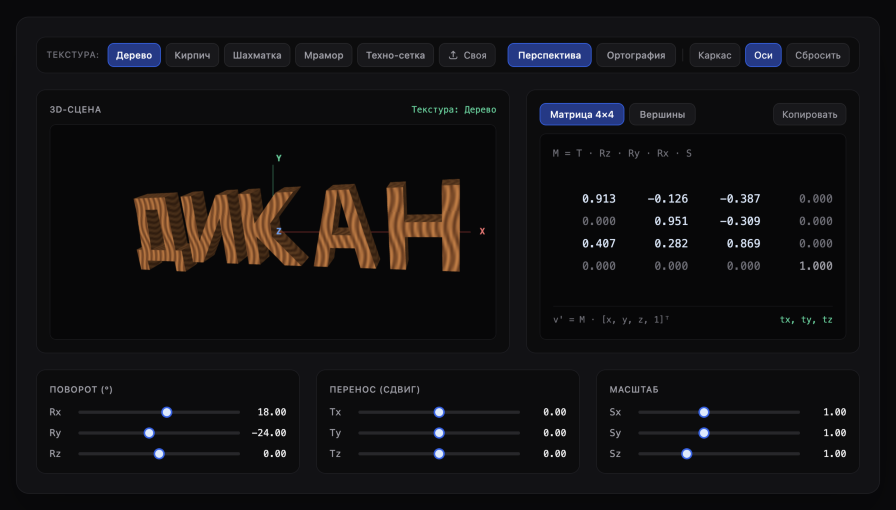
\includegraphics[width=0.72\textwidth]{../images/01_wood_perspective.png}
    \caption{Визуализация модели ДИКАН с текстурой дерева в перспективной проекции и матрицей $4 \times 4$}
\end{figure}

\begin{figure}[H]
    \centering
    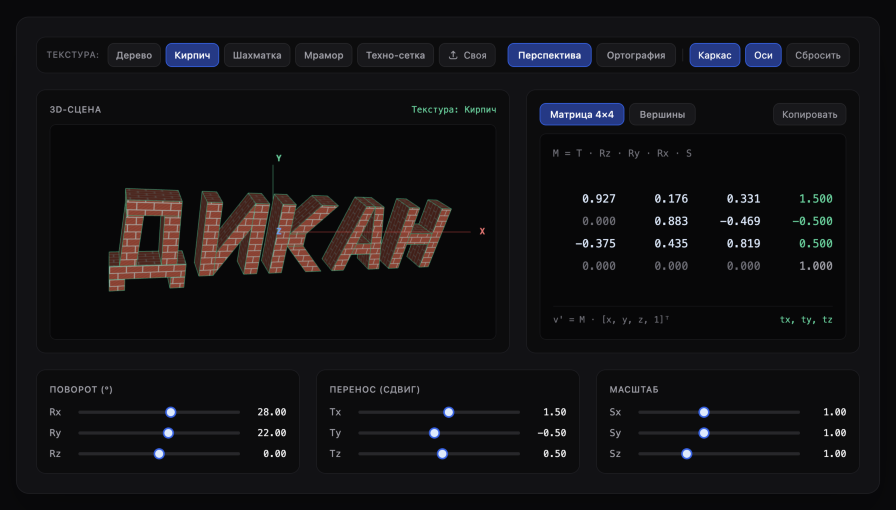
\includegraphics[width=0.72\textwidth]{../images/02_brick_wireframe.png}
    \caption{Текстура кирпича, включённый каркас рёбер и обновлённая матрица при переносе и повороте}
\end{figure}

\newpage

\begin{figure}[H]
    \centering
    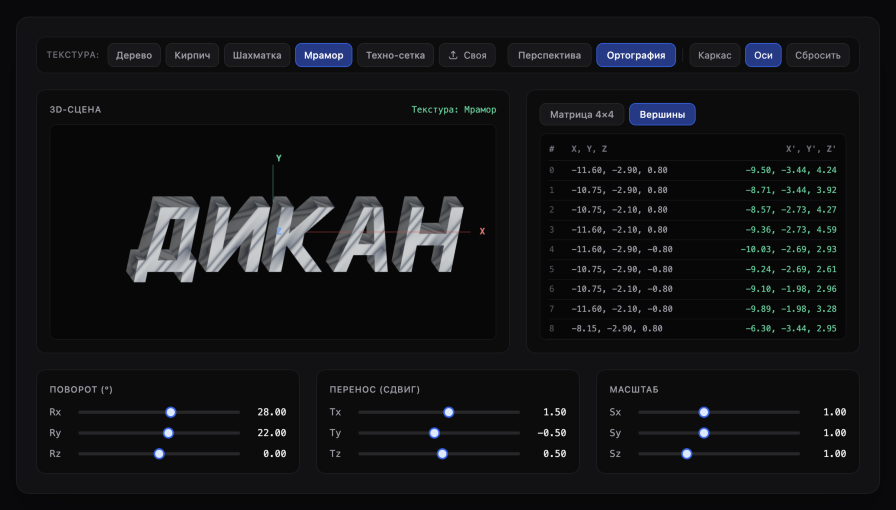
\includegraphics[width=0.72\textwidth]{../images/03_marble_ortho_vertices.png}
    \caption{Ортографическая проекция с текстурой мрамора и массив исходных и преобразованных вершин}
\end{figure}

% -------------------------------------------------------------
% ВЫВОДЫ
% -------------------------------------------------------------
\section*{7. Выводы}
\begin{enumerate}
    \item \textbf{Задание формы массивом вершин отделяет геометрию от преобразований.} Достаточно один раз описать 3D-объект через массив координат вершин и треугольные грани, после чего любые повороты, сдвиги и масштабирование сводятся к умножению координат на матрицу.
    \item \textbf{Матрицы $4 \times 4$ объединяют линейные преобразования и перенос.} Матрица $3 \times 3$ описывает только поворот и масштаб, но не позволяет выразить параллельный перенос. Переход к однородным координатам $(x, y, z, 1)$ сводит всю цепочку преобразований к одной итоговой матрице $M$, причём порядок перемножения ($T \cdot R \cdot S$) важен: сначала объект масштабируется и поворачивается вокруг своего центра, а потом сдвигается.
    \item \textbf{Для объёмного объекта одной UV-развёртки недостаточно.} Если на передней грани текстура ложится прямо по $(x, y)$, то на боковых стенках такой способ превращает рисунок в вытянутые полосы. Чтобы текстура не искажалась на торцах, боковым граням нужны отдельные UV-координаты вдоль длины ребра и глубины.
    \item \textbf{Восприятие объёма зависит от освещения, Z-буфера и типа проекции.} Без учёта угла между гранью и светом грани сливаются, а без Z-буфера дальние стенки перекрывают ближние. Перспективная проекция лучше передаёт глубину за счёт сужения вдаль, а ортографическая сохраняет параллельность линий и пропорции.
\end{enumerate}

\end{document}
